\documentclass[a4paper]{article}
\usepackage[T1]{fontenc}
\usepackage[scaled]{helvet}
\usepackage[margin=2cm]{geometry}
\usepackage{tikz}
\usepackage{circuitikz}
\usepackage{standalone}
\usepackage{xcolor}
\usepackage{colortbl}
\usepackage{multirow}

\renewcommand{\familydefault}{\sfdefault}
\begin{document}
\pagestyle{empty}
\begin{tikzpicture}
    \draw[] (0,1) -- (16,1) -- (16,25.7) -- (0,25.7) -- (0,1);
    \draw (0,25.7) node[anchor=north west](dfh){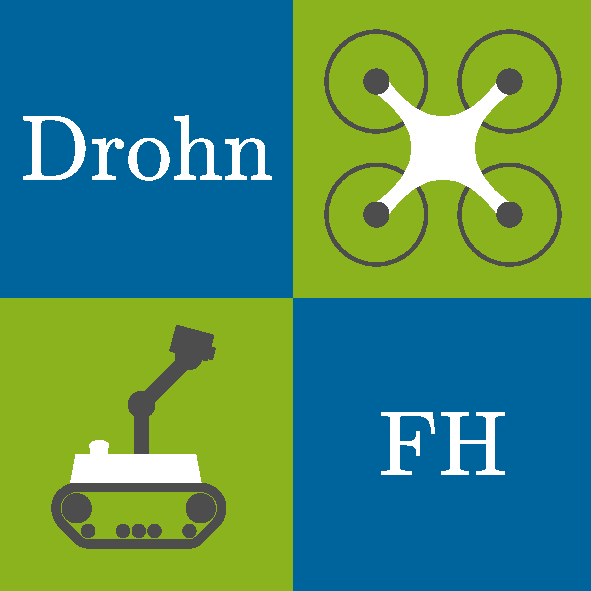
\includegraphics[height=2cm]{img/drohnfh.pdf}};
    \draw (16,25.7) node[anchor=north east](tw){
\includegraphics[height=2cm]{img/twlogo.pdf}};
    \draw[draw=none] (dfh.north east) -- (tw.north west) node[pos=0.5, anchor=north](ma23){
\includegraphics[height=2cm]{img/ma23.png}};
    \draw (0,23.4) -- (16,23.4);
    
    \draw (0,23) node[anchor=north west, align=left]{{\bfseries\huge Infineon DPS368 Breakout Board}\\[1em]{\bfseries\Large Digital XENSIV\textsuperscript{TM} Barometric Pressure Sensor Module}};
    
    \draw (0,21) node[anchor=north west, align=left]{{\bfseries\Large General Description}\\[1em]
                                                     {DPS368 is a miniaturized Digital Barometric Air Pressure Sensor robust against water, dust, and humidity.}\\
                                                     {It can be accessed via SPI or I\textsuperscript{2}C.}};
    \draw (0.15,19) -- (15.85,19);
    
    \draw (0,18) node[anchor=north west](SPI){\includestandalone[mode=buildnew, height=2cm]{img/dps368_SPI}};
    \draw (0,13.5) node[anchor=north west](I2C){\includestandalone[mode=buildnew, height=2.5cm]{img/dps368_I2C}};
    
    \draw (SPI.north west) node[anchor=south west,inner sep=0.2cm]{\large\bfseries Connection Diagram (SPI)};
    \draw (I2C.north west) node[anchor=south west,inner sep=0.2cm]{\large\bfseries Connection Diagram (I\textsuperscript{2}C)};
    
    \draw (SPI.north east) ++(0.7,0.9) -- ++(0,-4.2);
    \draw (SPI.north east) ++(0.7,-3.6) -- ++(0,-5.2);
    
    \draw (0.15,14.5) -- (15.85,14.5);
    \draw (0.15,9) -- (15.85,9);
    \draw (0.15,4.25) -- (15.85,4.25);
    \draw (0.15,3.25) -- (15.85,3.25);
    
    \draw (6,18.75) node[anchor=north west,align=left]{\scriptsize Write: First Byte is \{MSB=0, 7-bit Register Address\}\\
                                                          \scriptsize Read: First Byte is \{MSB=1, 7-bit Register Address\}\\
                                                          \scriptsize Supports SPI speeds up to 10~MHz.\\[1em]
                                                       };
    
    
    \draw (6,14.25) node[anchor=north west,align=left]{\scriptsize 7-bit I2C Address (AD0 floating): 0b1110111 = 0x77 \\
                                                        \scriptsize 7-bit I2C Address (AD0 pulled down): 0b1110110 = 0x76 \\
                                                        \scriptsize Supports I2C speeds up to 400~kHz as well as High-Speed Mode (up to 3.4 MBit/s).\\[1em]
                                                        };
    
    \draw (0,9) node[anchor=north west,align=left]{
    \large\bfseries Electrical Characteristics\\[0.5em]
    
    \begin{tabular}{|l|l|c|c|c|c|}
        \hline
        \rowcolor{gray!50} Parameter & Conditions & MIN & TYP & MAX & UNITS \\
        \hline
        \multicolumn{6}{|c|}{Supply Voltages}\\
        \hline
        VDD       &            & 1.7 &  & 3.6 & V \\
        \hline
        VDDIO     &            & 1.2 &  & 3.6 & V \\
        \hline
        \multicolumn{6}{|c|}{Supply Currents}\\
        \hline
        \multirow{3}{*}{Avg. Supply Current} & Pressure Meas @ 1Hz & & 1.7 & & µA \\
        \cline{2-6}
                                              & Temperature Meas @ 1Hz & & 1.5 & & µA \\
        \cline{2-6}
                                              & Standby & & 0.5& & µA \\
        \hline
    \end{tabular}
    \\[0.5em]
    
    \large\bfseries Further Details\\[0.25em]
    For further details, please consult the datasheet for the Infineon DPS368 sensor.\\[0.5em]
    
    \large\bfseries Acknowledgment\\
    \scriptsize This work was supported by the City of Vienna via the project ``Stadt Wien Kompetenzteam für Drohnentechnik in der Fachhochschulausbildung''\\[-0.25em]
    \scriptsize (MA23 Projekt Nr. 35-02)\\[0.5em]
    
    
    Version: 1.0 (2026-06-12)
    };
    
\end{tikzpicture}




\end{document}
